\documentclass{article}
\usepackage{amsmath}
\usepackage{amsthm}
\usepackage{algorithm}
\usepackage{algpseudocode}
\usepackage{amssymb}
\usepackage{graphicx}
\graphicspath{ {assets/} }

\usepackage{tikz}
\usetikzlibrary{shapes.geometric,arrows,fit,matrix,positioning}

\begin{document}

\title{Assignment 1 - Homework Exercises on I/O-Efficient Algorithms}
\author{
	Duy Pham - 0980384 \\
	Maciej Wiłkowski - 0927420 \\
	Pattarawat Chormai - 0978675 \\
}
\maketitle

\section*{IO.I-1}
\subsection*{(i)}
In this problem, we will show that when $m = M/B + 1$, if we have the optimal replacement policy, then it performs only $O(n/B + \sqrt(n))$ I/Os.\\

Indeed, when $M > B$ (which is obvious) and $m > M$, the array can be separated into blocks as being shown in figure \ref{fig:row-major}. \\

\begin{figure}
  \centering
  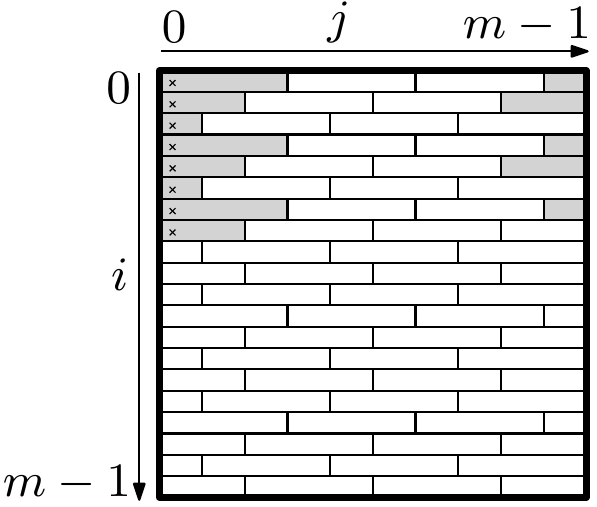
\includegraphics[width=0.5\textwidth]{row-major}
  \caption{Blocks loaded into an 2-dimensional array}
  \label{fig:row-major}
\end{figure}

Basically, we move in the column order, then each step in the first column requires an I/O. In each column, after filling the memory, there is still one more item left. This is when we need the replacement policy. The optimal replacement method (sometimes called $MIN$) removes the block that has the longest time to be reused again in the future. In this particular setting, the $MIN$ will remove the block which the last item has the smallest index. E.g. the $3^{rd}$ selected block in figure \ref{fig:row-major}.\\

If $B$ does not divides $m$, then each column in the array has $(m - 1) / B$ blocks which the last item index is that column index, which are also the blocks that have the longest time to be reused in the future. Moreover, these blocks are indeed never used again in the same row. Therefore, the number of I/Os that $MIN$ performs is equal to the number of I/Os that the row order performs, plus an extra number of I/Os for the remaining column of size $s < B$ (because $B$ does not divides $m$).\\

We have $m$ rows, and $m/B + 1$ I/Os for each row. Thus the number of I/Os is:

 $$(\frac{m}{B} + 1)m = O(\frac{n}{B} + \sqrt{n})$$

If $B$ divides $m$, then we do not have the distribution as being shown in figure \ref{fig:row-major}. Instead, all loaded blocks in a columns have the same ending index. Then the optimal replacement here is the Most Recently Used, that is, the policy evicts the latest used block. The array is now divided into $m / B$ columns of size $B$. Each such column requires $m$ I/Os for the first ``real'' column, and 1 I/O for each of the remaining columns. In general, the number of I/Os is:

$$\frac{m}{B}(m + B - 1) = \frac{m^2}{B} + \frac{m(B - 1)}{B} = O(\frac{n}{B} + \sqrt{n})$$

\subsection*{(ii)}
In case $m > 2M/B$ and $m$ is significantly larger than $M$, then there are more than $2M/B$ blocks for each column.\\

If we traverse the array in column-major order and the OS uses the optimal replacement strategy, then at the end of each column, all elements in the first $M/B $ blocks have been removed to get the space for the latest elements in the column. Therefore, whatever replacement method we use (even the optimal one), we cannot reuse any block when we move to the next column. Therefore, we need to load a new block every time we want to fetch a new item. Thus, the I/O complexity is $\Omega(n)$.\\

If the OS uses the Most Recently Used replacement policy, then we can keep $m/2$ items for the first column, but we have to load-and-clear every item in the remaining $m/2$ items. Therefore, the I/O complexity is still a factor of $m^2$, which is $\Omega(n)$.

\section*{IO.I-2}
\subsection*{(i)}
Let $T(n)$ denote IO's of the problem and $T_x$, $T_y$ and $T_z$ denote IO's of matrix $X$, $Y$ and $Z$ respectively.
For each cell in $Z$, we need
\begin{align*}
	T_x &\leq \frac{\sqrt{n}+2(B-1)}{B}\\
	T_y &\leq \sqrt{n} \\
	T_z &= 1
\end{align*}
Then, the total IO's we need for computing a cell is :
$$\frac{\sqrt{n}+2(B-1)}{B} + \sqrt{n} + 1$$
Therefore, the total IO's that we need to compute the product $Z=XY$ :
\begin{align*}
	T(n) &\leq ( \frac{\sqrt{n}+2(B-1)}{B} + \sqrt{n} + 1	)n\\
	&\leq \frac{n\sqrt{n}+2n(B-1)}{B} + n\sqrt{n} + n \\
	&= O(n\sqrt{n})
\end{align*}

\subsection*{(ii)}
If $Y$ is stored in $column-major$ order. For each cell, we will use $$T_y=\frac{\sqrt{n}+2(B-1)}{B}$$.
Therefore, the total IO's is
\begin{align*}
	T(n) &\leq ( 2\frac{\sqrt{n}+2(B-1)}{B} + 1	)n\\
	&\leq \frac{2n\sqrt{n}+4n(B-1)}{B} + n \\
	&= O(\frac{n\sqrt{n}}{B})
\end{align*}

\subsection*{(iii)}

% Image of X and Y how to find memory needed.

In order to compute sub-problem, all variables that we have in sub-problem should fit into main memory. 

Let $M_x$, $M_y$ and $M_z$ denote memory space that is required by $X$, $Y$ and $Z$ when computing a sub-problem

For each sub problem, we need
\begin{align*}
	M_x &= t(2t + 2(B-1)) \\
	M_y &= 2t(t+2(B-1))\\
	M_z &= t(t+2(B-1))
\end{align*}
Let $M$ denote the total memory we have. Then, we find IO's recursive base case which happens when all variables in sub-problem can fit into main memory.
\begin{align*}
M_x + M_y + M_z &\leq M \\
5n^2 + 6(B-1)n &\leq M
\end{align*}
Thus, we can formulate recurrence IO's complexity function of this algorithm.
\begin{align*}
	T(t) = \begin{cases}
	    \frac{5t^2 + 6(B-1)t}{B},& \text{if } 5t^2 + 6(B-1)t \leq M\\
	    4T(\frac{t}{2}),              & \text{otherwise}
	\end{cases}
\end{align*}
Hence, we have a general form of the function where $k$ is a depth of the recursive call.
\begin{align*}
	T(t) = 4^{k}T(\frac{t}{2^{k}})
\end{align*}
We know that if $\frac{n}{2^{k}} = 5n^2 + 6(B-1)n$ we will reach the base case. Then, we can find $k$.
\begin{align*}
	\frac{t}{2^k} &= 5t^2 + 6(B-1)t \\
	\frac{1}{2^k	} &= 5t + 6(B-1) \\
	2^k &= \frac{1}{5t + 6(B-1)} \\
	k\log2 &= log\frac{1}{5t + 6(B-1)} \\
	k &= log_2 \frac{1}{5t + 6(B-1)}
\end{align*}

Before we derive $T(t)$, we will denote $A$ as
$$ \frac{1}{5t + 6(B-1)}$$

Next, we can simply derive the IO's complexity of the algorithm.
\begin{align*}
	T(t) &\leq 4^{k}T(\frac{t}{2^{k}}) \\
	&\leq 4^{log_2 A}T\Big(\frac{t}{2^{log_2 A}}\Big) \\
	&\leq A^2T(\frac{t}{A}) \\
	&\leq A^2\Big( \frac{5\frac{t}{A}^2}{B} + \frac{6(B-1)\frac{t}{A}}{B} \Big) \\
	&\leq \frac{5t^2}{B} + \frac{6(B-1)t}{AB} \\
	&= O(\frac{t^2}{B})
\end{align*}

Therefore the IO's complexity of the algorithm is $O(t^2/B)$.

\subsection*{(iv)}

Claim. The algorithm from (iii) has better spatial locality.

To prove the claim, as we can see from (i), the algorithm does not use blocks of $Y$ effectively. When it fetches a block of $Y$, it uses only one variable and move on. In contrast, the algorithm from (iii) can use all variables in a block. Because all variables that it needs for execution sub-problem are in the main memory already.
\\\\
Claim : The algorithm from (iii) has better temporal locality. 

To prove the claim, assume $B_0$ is the first block of $Y$. In (i), the algorithm will need the block again when the algorithm finishes $m$ iterations while the algorithm from (iii) will need the block after $m/2$ iterations which is 2 time shorter than (i).

\section*{IO.1-3}
\subsection*{(i)}
The worst case of a binary search is when each step of comparison, we need to do an I/O to load the next center until the 2 consecutive centers are in the same block, which means the remaining array has to fit in 1 block. Suppose that after $k$ steps of binary searching, we reach that state, then:

$$2 \frac{n}{2^k} \leq B \iff \frac{n}{2^k} \leq \frac{B}{2}$$

Then,

$$k \geq log_2 \frac{2n}{B} $$

This means we have to do $log_2 \frac{2n}{B}$ I/Os before everything is inside the memory.

\subsection*{(ii)}
To avoid the case that we perform an I/O everytime we make a comparison, we can organize the blocks differently. Now we group all of the sorted centers to blocks first, then the other elements. In this way, when we make a comparison, the other centers are loaded also in the same block, so it reduces the number of I/Os performed.\\

There are $2log(n)$ centers. So under this grouping policy, we need to perform $log(n) / B$ number of I/Os to find an element using binary search.

\subsection*{(iii)}
Our proposed solution significantly increase the spatial locality. In the original approach, we load a block to read only 1 center. Meanwhile, in our solution, all items in a block are useful for the algorithm.\\

The temporal locality of the 2 approach is the same. It is because we never reuse the block again after reading it, in both methods.

\section*{IO.II-1}
Let $A = n\sqrt{n} / (M B)$, then the optimal policy performs $cA$ I/Os.\\

Suppose we perform the algorithm on a machine with $M' = M / 2$ memory. Then the optimal policy definitely performs $n\sqrt{n} / (\frac{M}{2} B) = 2cA$ I/Os. \\

According to theorem $5.3$ in the course notes, the LRU will perform the following number of I/Os when it is given a memory of $M$, while the optimal is given a memory $M' = M / 2 < M$:

$$LRU(M) \leq \frac{M}{M - M' + B} MIN(M')$$ \\
$$= \frac{M}{\frac{M}{2} + B} MIN(M')$$ \\ 
$$= \frac{2M}{M + 2B}2c\frac{n\sqrt{n}}{MB}$$ \\
$$= 4c\frac{n\sqrt{n}}{(M + 2B)B}$$ \\
$$\leq 4c\frac{n\sqrt{n}}{MB} = 4cA$$ \\ 

Let $c' = 4c$, then the LRU need at most $c'A$ I/Os.

\section*{IO.II-2}
\subsection*{(i)}
Let $n$ be the total number of items to be sorted, and $k = M/B - 1$ be the number of subarrays.\\

The complexity of the EM-MergeSort is the cost of the recurrence plus the cost of merging $k$ subarrays of size $n/k$ into an array of size $n$. \\ 

For each element, we have to perform $k-1$ comparisons to put it to the proper position in the final array. We have $n$ element in total, so the cost of merging is $O(n(k - 1)) = O(nk)$.\\

We can write the recurrence formula of the EM-MergeSort as follows:

$$T(n) = kT(n/k) + O(nk)$$

The base case is when $n = 1$, then $T(n) = 1$.\\

Analyzing this recurrence formula, we have:\\

\begin{equation*}
\begin{aligned}
&T(n) = k^2T(n/(k^2)) + 2.O(nk) \\
&= k^3T(n/(k^3)) + 3.O(nk) \\
&= \cdots \\
&= k^\alpha T(n/(k^\alpha)) + \alpha O(nk) \\
\end{aligned}
\end{equation*}


$T(n)$ reaches the base case when $n/(k^\alpha) = 1 \iff \alpha = \log_k n$, so the number of I/Os is:

$$T(n) = k^{\log_k n} (n/(k^{log_k n})) + \log_k n.O(nk) = n + \log_k n.O(nk) = O(nk\log_k n)$$

\subsection*{(ii)}
We propose another merging strategy as shown in algorithm \ref{alg:merge}.

\begin{algorithm}[h]
  \caption{Finding minimum row square cover}
  \label{alg:merge}
  \begin{algorithmic}
    \Require List of subarrays $S = {A_1, A_2, \cdots, A_k}$
    \Ensure Merged Array $A$

  \If{$k / 2 > 0$} 
  \State $A_{last} = A{k}$
  \State $k = k - 1$
  \EndIf
  \While{$SizeOf(S) > 1$}
  \State Construct $k/2$ pairs of subarrays $\{A_1, A_2\},\cdots, \{A_{k - 1}, A_k\}$
  \State Clear(S)
  \For{Each pair $\{A_i, A_j\}$}
  \State Merge $A_i$ and $A_j$ into $A_{ij}$
  \State Add $A_{ij}$ to S
  \EndFor
  \EndWhile

  \If{$A_{last}$ NOT NULL}
  \State Merge S[0] with $A_{last}$
  \EndIf

  \Return S[0]
\end{algorithmic}
\end{algorithm}

Now we analyze the complexity of the new merging strategy, and then the complexity of the EM-MergeSort using this as the main merging routine. \\

For each step, we reduce the number of pairs by 2. So it takes $O(\log k)$ steps to converge to 1 array.\\ 

For each pair of size $n/k$, it takes $O(2n/k)$ comparisons to merge them into 1. In each step of the merge, we perform $O(n)$ comparisons.\\

In general, the complexity of the merge step is $O(n\log k)$. So the recurrence formula of the K-way MergeSort is:

$$T(n) = kT(n/k) + O(n\log k)$$

We have:

\begin{equation*}
\begin{aligned}
T(n) &= k^2 T(n/(k^2)) + 2.O(n\log k) \\
&= k^3 T(n/(k^3)) + 3.O(n\log k) \\
&= \cdots \\
&= k^\alpha T(n/(k^\alpha)) + \alpha O(n\log k)
\end{aligned}
\end{equation*}

$T(n)$ reaches the base case when the problem size reaches 1. It takes $\log_k n$ steps to do so, then:

$$T(n) = n + \log_k n O(n\log k) = n + O(n\frac{log n\log k}{\log k}) = O(n\log n)$$

So our new merging strategy satisfies the condition.


\section*{IO.II-3}

If we assume that the algorithm runs in $ O(n) $ time it still impossible for it to work in  $ O(n/B) $ IOs. Supposedly a block $ B $ in the input array can contain $ n $ elements. For the algorithm to perform this amount of IOs we would need to assume that the values inside the block will be placed in the output array next to each other. Therefore we would need to assume the input array is already sorted. Since we cannot guarantee this kind of distribution we have to assume that in the worst case scenario we will $ n $ elements from a block will find its own places in $ n $ separate blocks in the output. Since in this optimistic case the number of IOs is O(n) we can assume it's impossible for them to be O(n/B).

\section*{IO.II-4}
Consider a permutation algorithm that does use additional memory blocks. We revise it a little bit so that all write operations are 
to blocks in A. We know that whenever we perform a write, there is at least 1 free block in A because it is a movement-only 
algorithm. Thus, whenever the algorithm perform a write to an external block, we perform an additional write to move it back to a
free block in A. After finishing the permutation task, we write these blocks back to the external memory. In this way, each block may require 3 I/O's. Therefore the number of possible states created by a write is $3\frac{n}{B} $. \\

\begin{itemize} 
  \item The total number of permutations of an array A of size $n$ is $n!$. In this problem, we do not care about the number of 
permutations inside a block. So we ignore $(B!)^{\frac{n}{B} }$ permutations. Then the total number of permutations available is 
$\frac{n!}{(B!)^{\frac{n}{B} }}$.
\item Because we write each block back to the main memory if it is written outside, one read can create a number of possible states as $\frac{n}{B} $
\item One write can create a number of possible states as $\frac{3n}{B} \binom MB$
\end{itemize}

Let $X^r$ denote the number of reads performed, and $X^w$ denote the number of writes. Since both initially and finally all elements are in the external memory, $X^r = X^w = \frac{X}{2}$. \\ 

Similar to the lecture notes, we come up with:

\begin{equation*}
  \begin{aligned}
  \frac{n!}{\big(B!\big)^{\frac{n}{B}}} &\leq \bigg(\frac{n}{B} \bigg)^{\frac{X}{2}} . \bigg(\frac{3n}{B} \binom MB\bigg)^{\frac{X}{2}} \\
  &= 3^{\frac{X}{2}}.\frac{n}{B}^X.\bigg(\binom MB\bigg)^{\frac{X}{2}} \\
  \iff X.\log \bigg(3^\frac{1}{2}.\frac{n}{B}.\bigg(\binom MB\bigg)^\frac{1}{2} \bigg) &\geq \log \bigg(\frac{n!}{(B!)^{\frac{n}{B}}}\bigg)
\end{aligned}
\end{equation*}

Similar to the course notes, we derive the following bound of the right-hand-side expression from Stirling's approximation:

$$\log \biggl(\frac{n!}{(B!)^{\frac{n}{B}}}\bigg) = \Omega(n\log(n/B))$$

For the left-hand-side expression, using the condition that $n < B\sqrt{\binom MB}$, and the inequality $\binom MB \leq 
\big(\frac{eM}{B}\big)^B$, we get:

\begin{equation*}
  \begin{aligned}
  \log \bigg(3^\frac{1}{2}.\frac{n}{B}.\bigg(\binom MB\bigg)^\frac{1}{2} \bigg) &< \log \bigg(3^\frac{1}{2} . \binom MB \bigg) \\
  &\leq \frac{\log 3}{2} + B \log \biggl( \frac{eM}{B} \bigg) \\
  &\leq 3B \log \big(\frac{M}{B}\big)
\end{aligned}
\end{equation*}

Hence:

\begin{equation*}
  \begin{aligned}
    X &\geq \frac{\log \biggl(\frac{n!}{(B!)^{\frac{n}{B}}}\bigg)}
    {log \bigg(3^\frac{1}{2}.\frac{n}{B}.\bigg(\binom MB\bigg)^\frac{1}{2} \bigg)} \\
    & = \frac{\Omega(n\log(n/B))}{3B \log \big(\frac{M}{B}\big)} \\
    & = \Omega \big( (n/B)\log_{M/B}(n/B)\big)
\end{aligned}
\end{equation*}



% !TEX root = ../main.tex

\tikzset
{
    treenode/.style = {circle, draw=black, align=center, minimum size=1cm},
}

\section*{IO.III-1}

\subsection*{(i)}
When the subarray fits into 1 block, then one of the subtree does not need any more I/Os and the other one needs one more I/O (because the next center is in a consecutive block).\\ 

The number of steps needed to reach such case is $\log(n/B)$. Then the error of the number of I/Os is $O(1)$. We have:
$$\#I/Os = \log(n/B) \pm O(1)$$

\subsection*{(ii)}
Instead of storing blocks as in-order traversal, we will separate the tree in to small subtrees of size B and store it into a block as shown in figure \ref{fig:blocking}.
\\\\
We know that the depth of the tree is $\log n$ and the depth of subtree is $\log B$. Therefore IO's complexity of root-to-leaf traversal is :
$$T(n) = \frac{\log n}{\log B} = \log_{B} n$$

As shown in figure \ref{fig:blocking}, this blocking strategy make the tree look similar to B-tree in a sense that
its nodes are grouped into subtrees and each subtree is comparable to a node in B-tree that can have more than 1 element.

\begin{figure}[t]
%\centering
{
    \begin{tikzpicture}[->,>=stealth', level/.style={sibling distance = 10cm/#1, level distance = 1.5cm}, scale=0.6,transform shape]
    \node [treenode] {$8$ \\ B1}
    child
    {
        node [treenode] {$4$ \\ B1} 
        child
        {
            node [treenode] {$2$ \\ B2} 
            child
            {
            		node [treenode] {$1$ \\ B2 }
            }
            child
            {
            		node [treenode] {$3$ \\ B2}
            }
        }
        child
        {
            node [treenode] {$6$ \\ B3} 
                        child
            {
            		node [treenode] {$5$ \\ B3 }
            }
            child
            {
            		node [treenode] {$7$ \\ B3}
            }
        }
    }
    child
    {
        node [treenode] {$12$ \\ B1} 
        child
        {
            node [treenode] {$10$ \\ B4} 
            child
            {
            		node [treenode] {$9$ \\ B4 }
            }
            child
            {
            		node [treenode] {$11$ \\ B4}
            }
        }
        child
        {
            node [treenode] {$14$ \\ B5} 
                        child
            {
            		node [treenode] {$13$ \\ B5 }
            }
            child
            {
            		node [treenode] {$15$ \\ B5}
            }
        }
    }
    ;
    \end{tikzpicture}
    \caption{An illustration of subtree blocking strategy when B=3 \label{fig:simple}}
    \label{fig:blocking}
}
\end{figure}

% !TEX root = ../main.tex
\section*{IO.III-2}

Let $P$ denote the sequence of operations $op_0, \cdots, op_{n-1}$ and $op_i = (i,type_i,x_i)$ where $i$ is timestamp,
$type_i \in \{ Insert, Delete, Search \}$ and $x_i$ is the value of $op_i$ . Suppose all $op_i \in P$ are stored in external memory already.
In order to report $Search$ operations in O$(SORT(n))$, we have to do following steps below.
\begin{enumerate}
    \item Sort $P$ by $x_i$ and $i$ in ascending order using EM-MergeSort
    \item Traverse through all $op_i \in P$
        \begin{itemize}
            \item if $type_i \in \{ Insert, Delete \}$ then $pv$ = $op_i$
            \item if $type_i \in \{ Search \}$ and $x_i$ is equal to $x_{pv}$ and $type_{pv}$ = Insert
                then report $op_i$ = Found
            \item otherwise report $op_i$ = Not Found
        \end{itemize}
\end{enumerate}

\textbf{Theorem.} This steps performs $O( SORT(n) )$ and report $Search$ operations correctly.
\begin{proof}
We first look at the number of I/O's that we need to perform such steps.
We know that $EM-MergeSort$ takes $O(SORT(n))$ I/O's and traversing sorted array takes $O(n/B)$ I/O's.
The total number of I/O's complexity is still $O(SORT(n))$. Secondly, this steps will always report correct result since
we sort $P$ by $x_i$ and $i$ in ascending order that means it will report as Found only when there is a $Insert$ operation
coming before $Search$ operation.
\end{proof}


% !TEX root = ../main.tex
\section*{IO.III-3}

\begin{algorithm}
  \caption{Coloring Undirected Graph}
  \label{alg:global_minimum}
  \begin{algorithmic}
    \renewcommand{\algorithmicrequire}{\textbf{Input:}}
    \renewcommand{\algorithmicensure}{\textbf{Output:}}
    \algnewcommand\algorithmicoperation{\textbf{Operation:}}
    \algnewcommand\Operation{\item[\algorithmicoperation]}
    \Require $G( V, E )$
    \Ensure Color of $v_i \in V$
    \Operation
    \State Convert $G$ into a DAG graph $G^*$ by directing every edge ( $v_i$, $v_j$ ) where $i < j$
    \State Initialise an array F[0..$n-1$], a min-priority queue $Q$
    \State Initialise a set of colour C[0..$d_{max}$]
    \For {$i$ := 0 to $n-1$}
    	\State Performs $Extract-Min$ operations on $Q$ until getting a pair whose priority $i' > i$
	\State Insert the extra extracted pair back to $Q$
	\State $f(v_i)$ := Choose one colour from C $\setminus$ \{ extracted pairs \}
	\State F[i] := $f(v_i)$
	    \For { each $j$ in $V[i].OutNeighbors$ }
	        \State Insert a pair ( $f(v_i)$, $j$ ) into $Q$
	   \EndFor
    \EndFor \\
    \Return F
  \end{algorithmic}
\end{algorithm}
\textbf{Theorem.} The algorithm performs $O( SORT(|V|+|E|) )$ and returns valid solution.

\begin{proof}
    Let denote $N_{in}$ a set of in-neighbor of $v_i \in V$. We observe that each iteration the algorithm performs
    $$2O( SORT(1 + |N_{in}(v_i)| ))$$
One from $Extract-Min$ operation and the other from $Insertions$. \\
Thus, the total I/O's complexity  is :
\begin{align*}
    T_{io}(G(V,E)) &= \sum^{n-1}_{i=0}{O( 1 + |N_{in}|)(v_i)} \\
    &= O( SORT( |V|+|E| ))
\end{align*}

To prove that the algorithm returns valid solution. We first argue that the algorithm does not use more than $d_{max} + 1 $ colours .
Secondly, there are no 2 adjacent nodes having same colour because each time it picks a colour the list of colours is subtracted by colours used for its in-neighbors.

\end{proof}


\end{document}
